
\documentclass[12pt,epsfig,color,russian]{article}
\usepackage[russian]{babel}
\usepackage{epsfig}
\usepackage{color}

\topmargin=0cm
\hoffset -30mm
\voffset -12mm
\setlength{\unitlength}{1mm}
\parindent=10mm
\textheight=250mm
\textwidth=185mm
\pagestyle{empty}

\begin{document}
\sf\Large


\centerline{\underline{\Huge\bf Элементы СТО}}
{\sl И.Е.Иродов, Основные законы механики, глава 6}

Представления о пространстве и времени в классической (ньютоновской) механике:
\begin{enumerate}
\item Пространство -- Евклидово и имеет 3 измерения.
\item $\exists$ время, не зависящее от пространства (но его измерение связано с законами движения)
\item Размеры тел и промежутки времени одинаковы для всех систем отсчета (Ньютон: пространство и время -- абсолютны!)
\item справедлив 1зН: $\exists$ инерциальные системы, и в них $\exists$ механический принцип относительности Галилея
\item Из (1--4) вытекают преобразования Галилея:\\
  \begin{picture}(180,50)(0,0)
   %\put(0,0){\framebox(180,50)[b]{}}
   \put(125,0){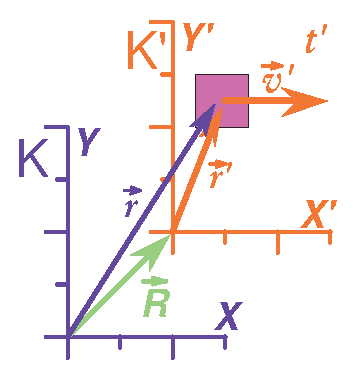
\includegraphics{GP007F01.eps}}
   \put(0,0){\makebox(0,0)[bl]{\parbox{120mm}{
   Если система {\color{red}K'}
   описывается радиус-вектором {\color{green} $\vec{R}$}
   относительно системы {\color{blue}K}, то событие, опи\-сываемое
   в этой системе радиус-вектором {\color{red}$\vec{r'}$},
   будет в системе {\color{blue}K} иметь радиус-вектор \\ ${\color{blue}\vec{r}}={\color{green}\vec{R}}+{\color{red}\vec{r'}}$. При этом {\color{blue}$t$}={\color{red}$t'$} и, соответственно,
   ${\color{blue}\dot{\vec{r}}}={\color{green}\dot{\vec{R}}}+{\color{red}\dot{\vec{r'}}}$, то есть, ${\color{blue}\vec{v}}={\color{green}\vec{V}}+{\color{red}\vec{v'}}$
   или ${\color{blue}\vec{r}}={\color{green}\vec{V}}t+{\color{red}\vec{r'}}$
   }}}
  \end{picture}
\item $\exists$ механический принцип относительности Галилея
\item $\exists$ принцип дальнодействия: все взаимодействия передаются мгновенно
\end{enumerate}
\rule{190mm}{0.3mm}
Вопрос: $\exists$ ли абсолютная система отсчета? $\exists$ ли явления (не механи\-че\-с\-кие), которые отличались бы в разных инерциальных системах?

{\bf Природа света:} Считалось, что это колебания некой упругой среды наподобие воздуха ("эфир"). Но такая среда не может быть неподвижной относительно сразу всех инерциальных систем $\Rightarrow$ должна быть одна "аб\-со\-лют\-ная" система! Эфир?...
\newpage
{\bf \underline{Опыт Майкельсона и Морли}}\\
  \begin{picture}(190,50)(0,0)
   %\put(0,0){\framebox(190,50)[b]{}}
   \put(120,0){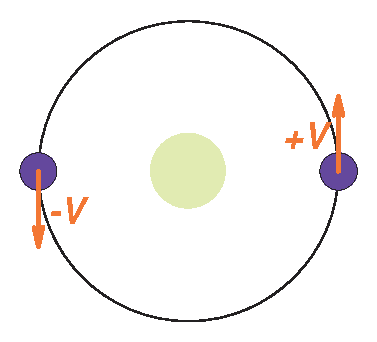
\includegraphics{GP007F02.eps}}
   \put(0,10){\makebox(0,0)[bl]{\parbox{110mm}{
Скорость света $c\simeq$ 300 000 км/с \\
(c 1983 года $c\equiv2.99792458\times10^{8}$ м/с)\\
Орбитальная скорость Земли $V\simeq$ 30 км/с\\
$V/c\simeq10^{-4}$, и можно попытаться увидеть результат сложения скоростей $c\pm V$.
   }}}
  \end{picture}\\
  \begin{picture}(190,100)(0,0)
   %\put(0,0){\framebox(190,100)[b]{}}
   \put(0,0){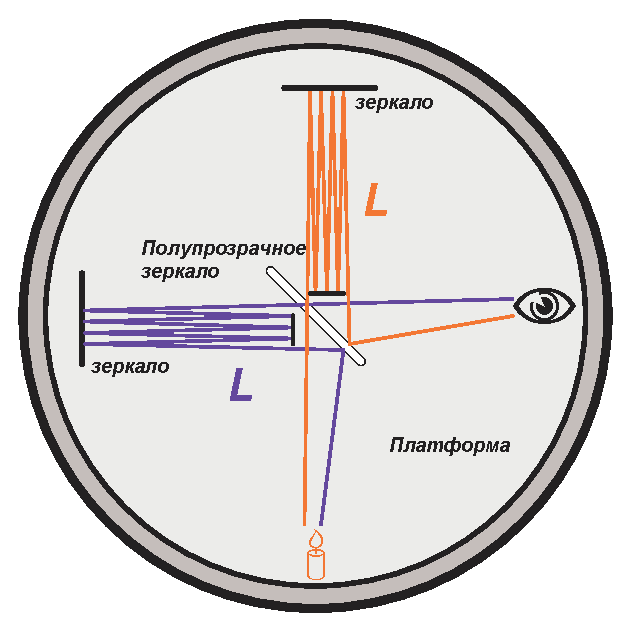
\includegraphics{GP007F03.eps}}
   \put(190,93){\makebox(0,0)[rt]{\parbox{85mm}{
1887 год. Гранитная платформа, плавающая в ванне со ртутью (убирает вибрации и облегчает вращение). {\color{blue}Первый} луч проходит путь {\color{blue}$nL$} на запад и {\color{blue}$nL$} на восток, а {\color{red}второй} -- {\color{red}$nL$} на север и {\color{red}$nL$} на юг. Пусть Земля в эфире движется на юг со скоростью $V$. В лабораторной системе (л.с.): эфир движется на север. Тогда в л.с. скорость света при движении луча на север $v_N=c+V$, на юг
   }}}
  \end{picture}\\
 $v_S=c-V$, на восток и на запад $v_O=v_W=\sqrt{c^2-V^2}$. Время, потраченное на весь путь первым лучем:
 \vspace{-5mm}
 \begin{displaymath}
 \hspace{20mm}T_1=T_O+T_W=\frac{nL}{v_O}+\frac{nL}{v_W}=\frac{2nL}{\sqrt{c^2-V^2}}
  =\frac{2nL}{c\cdot\sqrt{1-(V/c)^2}}\vspace{-5mm}
 \end{displaymath}
 Время, потраченное на весь путь вторым лучем:
 \vspace{-2mm}
 \begin{displaymath}
 T_2=T_N+T_S=\frac{nL}{v_N}+\frac{nL}{v_S}=\frac{nL}{c+V}+\frac{nL}{c-V}
 =\frac{2nLc}{c^2-V^2}=\frac{2nL}{c\cdot\left(1-(V/c)^2\right)}\vspace{-2mm}
 \end{displaymath}
 Разность путей, пройденных обоими лучами \underline{\bf в эфире}:
 \begin{displaymath}
 \Delta L=cT_2-cT_1=
\frac{2nL}{\left(1-(V/c)^2\right)}-\frac{2nL}{\sqrt{1-(V/c)^2}}\simeq nL\left( V/c\right)^2
\simeq12\;\texttt{нм}
 \end{displaymath}\vspace{-2mm}
При повороте платформы на 90$^\circ$ должно $\Delta L \leftrightarrow - \Delta L$, но никакой разности хода $2\Delta L\simeq0.04\lambda$ обнаружено не было!\\
Могло, конечно, {\bf случайно} оказаться, что в тот момент было V=0. Тогда через полгода должно быть V=60 км/с. Повторили -- безрезультатно!

Выводы: 1) эфир никак не обнаружить  2) Скорость света не зависит от скорости источника.

Максвелл: скорость распространения эл.-маг. поля в пустоте c=const безотносительно к системам отсчета(?!)

Лоренц (1892): сокращение длины тела в направлении движения.

Пуанкаре (1905): принцип относительности Галилея надо рас\-про\-стра\-нить на {\bf все явления, включая электродинамику}, а не только на механику. "Преобразования Лоренца". Одновременность событий не абсо\-лют\-на. 4-мерный интервал $r^2+(ict)^2$ -- инвариант преобразований Лоренца. Скорость распространения гравитации в эфире = с.

Эйнштейн (1905): Зачем эфир, если он ненаблюдаем? 2 постулата: спец. принцип относительности и постоянство с.

Планк (1906) и Эйнштейн (1907): релятивистская динамика и тер\-мо\-ди\-на\-мика.

Минковский (1907): математическая модель СТО (геометрия 4-мер\-но\-го псевдоевклидова пространства.

Эйнштейн (1911-1916): ОТО (гравитация как проявление кривизны пространства-времени).

Неужели нельзя разогнать что-то до скорости >c? Эксперимент Бер\-тоц\-ци на ускорителе электронов Ван-де-Граафа:\\
  \begin{picture}(190,80)(0,0)
   %\put(0,0){\framebox(190,30)[b]{}}
   \put(10,40){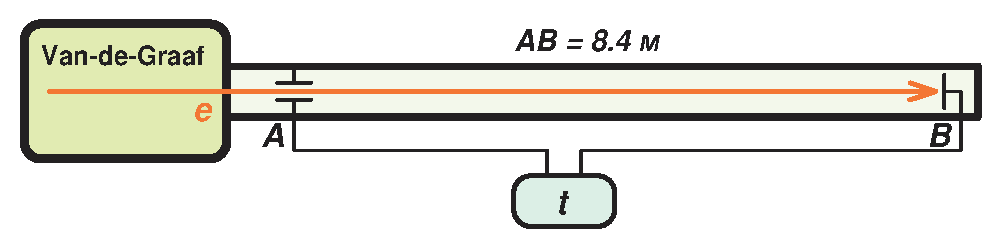
\includegraphics{GP007F04.eps}}
   \put(10,0){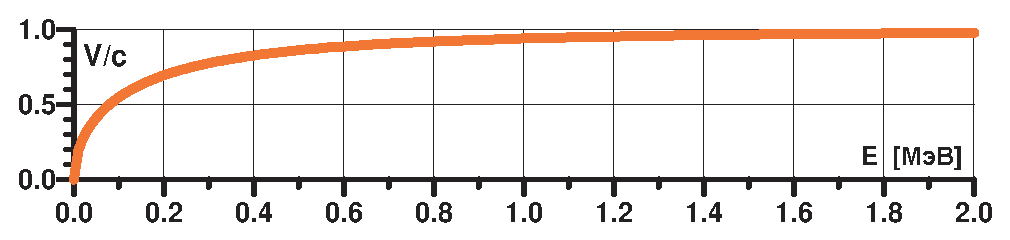
\includegraphics{GP007F05.eps}}
  \end{picture}\\


\underline{\bf ПОСТУЛАТЫ Эйнштейна} (он сложил их вместе):
\begin{enumerate}
\item Справедлив принцип относительности Эйнштейна -- расширение прин\-ци\-па Галилея.
\item Скорость света не зависит от скорости источника во всех инерциальных системах.
\item Пространство и время однородны; пространство -- изотропно.
\end{enumerate}
Если пренебречь гравитацией (а это учитывается в ОТО), то СТО выпол\-ня\-ет\-ся с точностью не хуже $10^{-12}$.\\

Раз c=const, то преобразования Галилея для скоростей НЕ ВЕРНЫ.
  \begin{picture}(190,45)(0,0)
   %\put(0,0){\framebox(190,40)[b]{}}
   \put(70,0){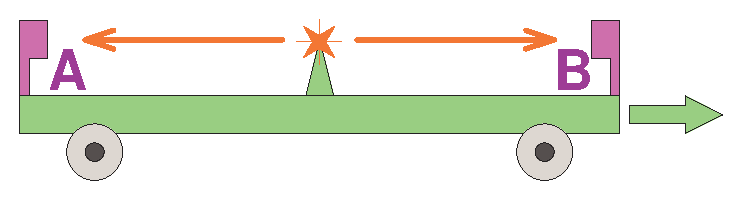
\includegraphics{GP007F06.eps}}
   \put(0,0){\makebox(0,0)[bl]{\parbox{65mm}{
   На тележке, едущей впра\-во, вспыхивает лампочка. В системе тележки свет до фотоэлементов A и B доходит одновременно.
   }}}
  \end{picture}

В л.с. пока свет летит, фотоэлемент A к нему приблизится и поймает сигнал раньше, чем B.

 То есть, ОДНОВРЕМЕННОСТЬ событий -- тоже относительна!

 Рассмотрим систему $K'$, движущуюся относительно покоящейся сис\-темы $K$ со скоростью $V$ в направлении оси $x$.

 Вместо преобразований Галилея $\Rightarrow$ преобразования Лоренца.
 \begin{displaymath}
 \begin{array}{lc|cl}
 x'=x-Vt &&\hspace{5mm}& x'=\frac{x-Vt}{\sqrt{1-V^2/c^2}}\rule[-5mm]{0mm}{10mm}\\
 y'=y    &&& y'=y\\
 z'=z    &&& z'=z\\
 t'=t    &&& t'=\frac{t-Vx/c^2}{\sqrt{1-V^2/c^2}}\rule[-6mm]{0mm}{15mm}\\ \hline
 \texttt{длина r}&&&\texttt{интервал s}\\
 r^2=x^2+y^2+z^2&&&s^2=-c^2t^2+x^2+y^2+z^2\\ \hline
 \texttt{пространство \{x,y,z\} + время \{t\}}&&&\texttt{4-континуум \{ict,x,y,z\}}
 \end{array}
 \end{displaymath}\\
  \begin{picture}(190,45)(0,0)
   %\put(0,0){\framebox(190,45)[b]{}}
   \put(0,0){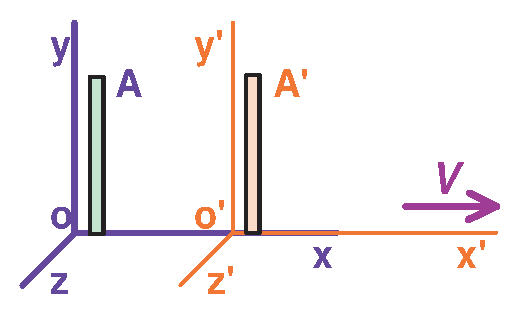
\includegraphics{GP007F07.eps}}
   \put(190,0){\makebox(0,0)[br]{\parbox{100mm}{
    Пусть в двух системах есть по вер\-ти\-каль\-ному стержню одинаковой длины ($OA\!\parallel\! y$) и ($O'A'\!\parallel\! y'$). Совпадают ли их длины с точки зрения другой системы? Да. Когда системы в какой-то момент поравняются, мы это увидим. $\Rightarrow {\color{blue}y}={\color{red}y'}$.
   }}}
  \end{picture}

  \centerline{\fbox{\bf\color{blue}Поперечные размеры Лоренц-инвариантны }}
  \vspace{5mm}
  Теперь превратим стержень в "световые часы": свет бегает вдоль стержня, отражаясь от концов, а мы считаем число пробегов.\\
  \begin{picture}(190,50)(0,0)
   %\put(0,0){\framebox(190,50)[b]{}}
   \put(0,0){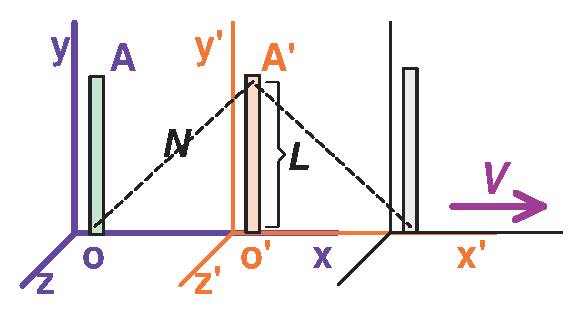
\includegraphics{GP007F08.eps}}
   \put(190,0){\makebox(0,0)[br]{\parbox{92mm}{
    В движущейся системе длина од\-но\-го пробега $L\!=\!(O'A')$, и он занимает время $t'=L/c$. С точки же зрения покоящейся системы, вместо катета $L$ надо брать диагональ $N$, и про\-бег займет большее время $t\!=\!\frac Nc$, причем
   }}}
  \end{picture}
  \begin{displaymath}
  \left(Vt\right)^2+L^2=(ct)^2\hspace{10mm}\Rightarrow\hspace{10mm}
  t=\frac{t'}{\sqrt{1-\left(V/c\right)^2}}\hspace{10mm}\Rightarrow\hspace{10mm}
  {\color{blue}t}\geq {\color{red}t'}
  \end{displaymath}
\\
  \centerline{\fbox{\bf\color{blue}Движущиеся часы идут медленнее, чем покоящиеся}}
  \begin{picture}(190,80)(0,0)
   %\put(0,0){\framebox(190,80)[b]{}}
   \put(70,0){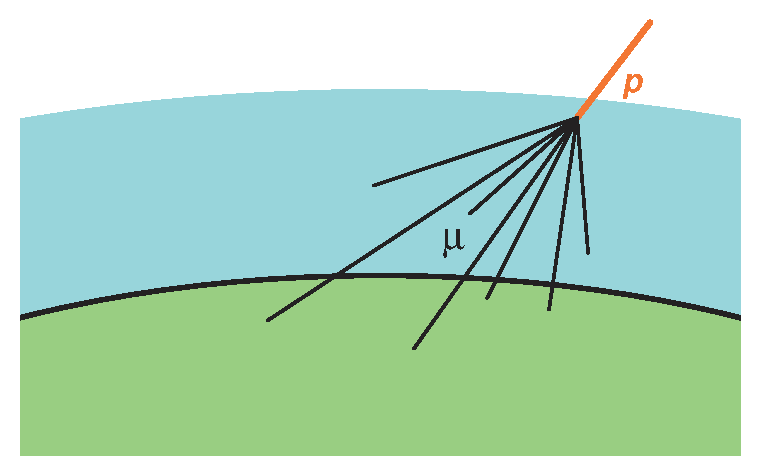
\includegraphics{GP007F09.eps}}
   \put(0,0){\makebox(0,0)[bl]{\parbox{65mm}{
    Покоящийся мюон живет $\tau\!\simeq\!2$ мкс; за это время он не смог бы пролететь более 600 метров, даже двигаясь с $V\!\simeq\! c$. Од\-на\-ко, рождающиеся на высоте 20-30 км мюоны легко достигают земной поверхности и вредят экспериментаторам...
    }}}
  \end{picture}
\\
  \begin{picture}(190,55)(0,0)
   %\put(0,0){\framebox(190,55)[b]{}}
   \put(0,0){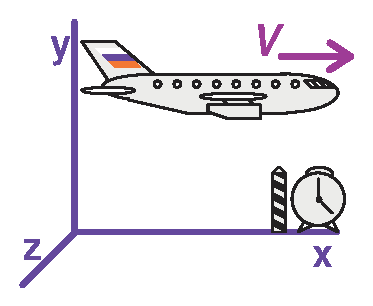
\includegraphics{GP007F10.eps}}
   \put(185,0){\makebox(0,0)[br]{\parbox{120mm}{
   Пусть теперь самолет движется вдоль оси $x$. В покоящейся системе поставим пограничный столб с часами и засечем время $t$ между моментами, когда со столбиком поравняются сначала кокпит, а затем киль самолета. Тогда его длина для стоящего возле столба погранич-
    }}}
  \end{picture}
\\
ника покажется равной $L=Vt$. У пилота нет возможности вылезти на лету и измерить длину своей машины, но он связался по рации с пограничником и узнал о показаниях часов. Будучи достаточно образован\-ным, пилот знает об эффекте замедления времени, а также о полном равноправии систем отсчета. Поэтому он считает, что часы пограничника идут медленнее (ведь они вместе со столбом движутся назад относительно самолета!) в $1/\sqrt{1-\left(V/c\right)^2}$ раз. Во столько же раз длина самолета оказыва\-ется больше с точки зрения пилота, чем это показалось пограничнику.\\
  \centerline{\fbox{\bf\color{blue} Размеры тела сокращаются в направлении движения}}
\vspace{1mm}

Попробуем вывести преобразования Лоренца для перехода от инерци\-аль\-ной системы $K$ к движущейся относительно нее вдоль оси $X$ со скорос\-тью $V$ инерциальной системе $K'$. Пространство и время однородны $\Rightarrow$   единица длины и единица времени одинаковы в любой точке пространства и в любой момент времени $\Rightarrow$ преобразования должны быть линейны:\vspace{-1mm}
\begin{equation}\label{Eq.1}
\left\{ \begin{array}{ccc}
        x'&=&Ax+Bt\\
        t'&=&Mx+Nt
        \end{array}\right.\hspace{10mm}\rightarrow\;\;\;\texttt{Найдем}\;\;\;\; A,B,M,N
\vspace{-2mm}\end{equation}\vspace{-2mm}
Перемещение вдоль оси $X$ в системе $K'$:\vspace{-2mm}
\begin{displaymath}
\Delta x'=x'_2-x'_1=A(x_2-x_1)+B(t_2-t_1)=A\Delta x+ B\Delta t
\end{displaymath}\vspace{-2mm}
Промежуток времени в системе $K'$:\vspace{-2mm}
\begin{displaymath}
\Delta t'=t'_2-t'_1=M(t_2-t_1)+N(x_2-x_1)=M\Delta x+ N\Delta t
\end{displaymath}\vspace{-2mm}
Учитывая, что скорости $v$ и $v'$ относительно систем $K$ и $K'$, соответственно, равны $v={\Delta x}/{\Delta t}$ и $v'={\Delta x'}/{\Delta t'}$, получим:\vspace{-2mm}
\begin{equation}\label{Eq.2}
v'=\frac{\Delta x'}{\Delta t'}=\frac{A\Delta x+ B\Delta t}{M\Delta x+ N\Delta t}=\frac{Av+B}{Mv+N}
\end{equation}
Рассмотрим некоторые частные случаи. Например, точка покоится в сис\-теме $K'$. Тогда $v'$=0, $v$=$V$. Подставив это в (\ref{Eq.2}), получим:
\begin{equation}
0=\frac{AV+B}{MV+N}\hspace{10mm}\Rightarrow\;\;\;\fbox{$B=-AV$}
\end{equation}
Пусть теперь точка покоится в системе $K$. Тогда $v$=0, $v'$=$-V$. Подставим в (\ref{Eq.2}):\vspace{-4mm}
\begin{equation}
-V=\frac{A\cdot0+B}{M\cdot0+N}=\frac BN=-\frac{AV}N\hspace{10mm}\Rightarrow\;\;\;\fbox{$N=A$}
\end{equation}
Теперь пусть в системе $K'$ распространяется свет. Тогда $v'$=$v$=$c$. Под\-ста\-вим в (\ref{Eq.2}):\vspace{-4mm}
\begin{equation}
c=\frac{Ac-AV}{Mc+A}\hspace{10mm}\Rightarrow\;\;\;\fbox{$M=-AV/c^2$}
\end{equation}
С учетом всего этого, формула (\ref{Eq.2}) превращается в\\[3mm]
{\color{blue} \parbox{180mm}{
\centerline{\fbox{\bf формулу сложения скоростей:}}
\begin{displaymath}
v'=\frac{v-V}{1-\frac{vV}{c^2}}\hspace{20mm}v=\frac{v'+V}{1+\frac{v'V}{c^2}}
\end{displaymath}
}}\\
\fbox{\parbox{190mm}{\sl Пример: две частицы летят навстречу друг другу со скоростями $+\frac 34c$ и $-\frac 34c$. Какова их встречная скорость? Свяжем систему $K'$ с первой частицей ($V=+\frac 34c$). Тогда с точки зрения этой первой частицы, скорость второй будет вовсе не $(\frac 34+\frac 34)c=1.5c$, а
\vspace{-3mm}
\begin{displaymath}
v'=\frac{-\frac 34c-\frac 34c}{1-\frac{-9c^2}{16c^2}}=\frac{-\frac 32 c}{\frac{25}{16}}=
-\frac{24}{25}c=-0.96c
\end{displaymath}}
\vspace{-3mm}
}\\[5mm]
\noindent
Теперь подставим найденные значения $B,M,N$ в изначальные ф-лы (1)
\vspace{-2mm}
\begin{displaymath}
\left\{ \begin{array}{ccc}
        x'&=&A(x-Vt)\\
        t'&=&A\left(t-\frac{Vx}{c^2}\right)
        \end{array}\right.
\end{displaymath}
Поскольку пространство изотропно, то можно считать, что не $K'$ движется со скоростью $V$, а $K$ движется со скоростью $-V$. Тогда получим
\vspace{-2mm}
\begin{displaymath}
\left\{ \begin{array}{ccc}
        x&=&A(x'+Vt)\\
        t&=&A\left(t'+\frac{Vx'}{c^2}\right)
        \end{array}\right.
\end{displaymath}
\vspace{-2mm}
\newpage
"скрестив" эти четыре равенства, получим уравнение для $A$:
\begin{displaymath}
x=A^2\left(x-Vt+Vt-\frac{V^2x}{c^2}\right)=xA^2\left(1-\frac{V^2}{c^2}\right)
\end{displaymath}
Поделив это на $xA^2$, найдем значение $A$:\\
\centerline{
\fbox{\parbox{170mm}{
\vspace{-2mm}
\begin{displaymath}
A={\color{blue}\frac 1{\sqrt{1-\frac{V^2}{c^2}}}}\;\;\;\;\;\equiv\;\;\;\;\; {\color{blue}\gamma}\;\;\;\;\;\equiv\;\;\;\;\;{\color{blue}\texttt{Лоренц-фактор}}\geq 1
\vspace{-2mm}
\end{displaymath}
}}}
С учетом этого, видим, что равенства  представляют собой не что иное как преобразования Лоренца (что и требовалось)!\\

Хотя одновременность событий и относительна, но {\bf причинно-след\-ствен\-ная связь} преобразованиями Лоренца не нарушается. Причина и следствие: причина всегда раньше, и без нее следстве невозможно.

Причина: в момент времени $t_1$ в точке $x_1$ произведен выстрел. След\-ствие: в момент $t_2$ в точке $x_2$ пуля со скоростью $v$ пробивает мишень.\\
  \begin{picture}(190,38)(0,0)
   %\put(0,0){\framebox(190,35)[b]{}}
   \put(15,0){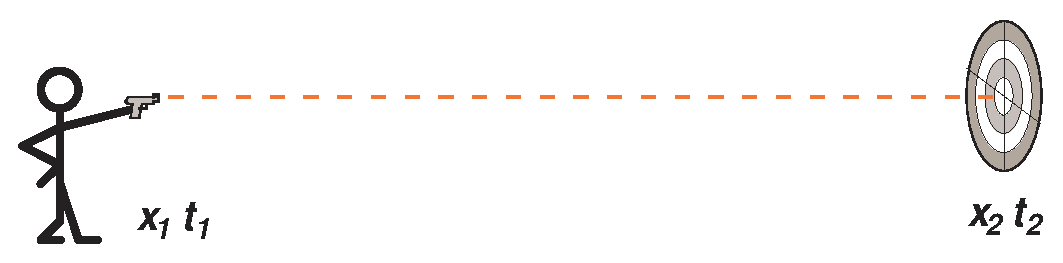
\includegraphics{GP007F11.eps}}
   \put(95,15){\makebox(0,0)[b]{$v=(x_2-x_1)/(t_2-t_1)$}}
  \end{picture}
\\
Предположим, что есть какая-то система отсчета $K'$, движущаяся со ско\-ростью $V$. В ней интервал между выстрелом и попаданием
\begin{displaymath}
 \Delta t'=t'_2-t'_1=\frac{t_2-t_1-\frac{V}{c^2}(x_2-x_1)}{\sqrt{1-(V/c)^2}}=
 (t_2-t_1)\frac{1-\frac{vV}{c^2}}{\sqrt{1-(V/c)^2}}=\Delta t\cdot\xi
\end{displaymath}
Поскольку $|v|\leq c$ и $|V|< c$, то множитель $\xi$ всегда положителен, $\Rightarrow$ знаки $\Delta t'$ и $\Delta t$ совпадают, то есть, действительно не найдется такой инерциальной системы, по отношению к которой причина и следствие поменялись бы местами.\\

\underline{\bf Интервал} $s$ между событиями 1 и 2:
\begin{displaymath}
s_{12}^2\equiv x^2+y^2+z^2-c^2t^2 = L^2-c^2t^2,
\end{displaymath}
где $L$ -- расстояние, а $t$ -- время между событиями 1 и 2. В системе $K'$:
\begin{displaymath}
s'^2=x'^2+y'^2+z'^2-c^2t'^2 =
\frac{(x-Vt)^2}{1-V^2/c^2}+y^2+z^2-
\frac{c^2(t-Vx/c^2)^2}{1-V^2/c^2}=
\end{displaymath}
\begin{displaymath}
=\ldots=
\frac{(x^2-c^2t^2)(1-V^2/c^2)}{1-V^2/c^2}+y^2+z^2=s^2
\end{displaymath}
\centerline{\fbox{\bf\color{blue}
Преобразования Лоренца не меняют длину интервала
}}
\vspace{2mm}\\
В чем смысл интервала? Лучше всего представить дело так, что вместо 3 пространственных осей ($X,Y,Z$) и одной временн\'{о}й оси ($T$), существуют 4 равноправные взаимно-ортогональные обобщенные оси $X_0,X_1,X_2,X_3$, причем обобщен\-ные координаты любого события записываются как 4-мерный вектор $\vec{x}$ с составляющими $x_\mu$ ($\mu=0\ldots3$):
\begin{equation}\label{Eq.Int}
 \vec{x}=\left\{\begin{array}{c}
                 x_0\\ x_1\\ x_2\\ x_3
                \end{array}\right\}=
\left\{\begin{array}{c}
                 ict\\ x\\ y\\ z
                \end{array}\right\};\;\;\;\;\;\;\;|x|^2 = \sum_{\mu=0}^3x_\mu^2
\end{equation}
Забыв на время об $y$- и $z$-составляющих, нарисуем "диаграмму Минковского".
\\
  \begin{picture}(190,91)(0,0)
   %\put(0,0){\framebox(190,90)[b]{}}
   \put(105,0){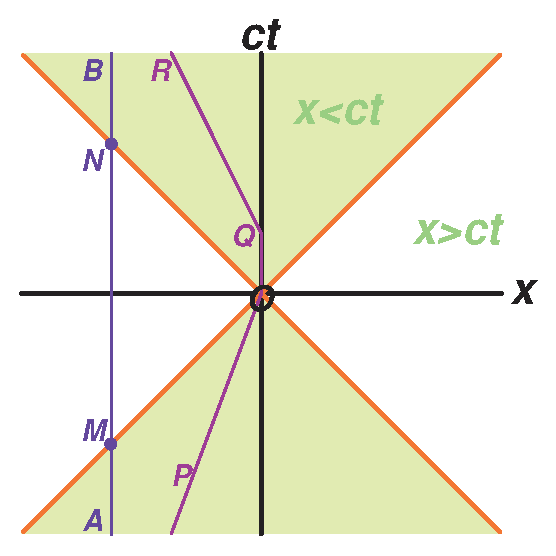
\includegraphics{GP007F12.eps}}
   \put(0,90){\makebox(0,0)[tl]{\parbox{100mm}{
   Начало координат -- это мы, то есть, {\bf здесь} ($x$=0) и {\bf сейчас} ($t$=0). Все остальные точки -- это события, ко\-то\-рые были ($t$<0) и будут ($t$>0) в разных закоулках Вселенной. Диагонали -- мировые линии света от нашей лампочки. Прямая $AB$ -- мировая линия покоящегося объекта. Он сможет получить нашу телеграмму только на участке $NB$.  $POQR$ -- другой объект приблизился, побудет в гостях и удалится обратно.
   }}}
  \end{picture}
\\
{\sl (Ч.Киттель, В.Найт, М.Рудерман. Берклеевский Курс Физики. Механика.)}
\\
  \begin{picture}(190,90)(0,0)
   %\put(0,0){\framebox(190,90)[b]{}}
   \put(0,0){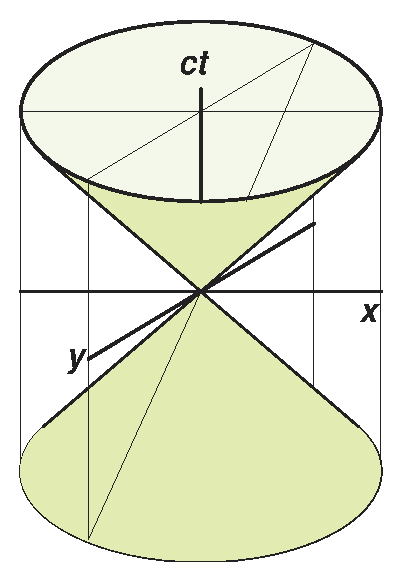
\includegraphics{GP007F13.eps}}
   \put(190,90){\makebox(0,0)[tr]{\parbox{120mm}{
   Если теперь вспомнить еще об одной про\-стран\-ственной координате ($y$), то вместо плоской ди\-а\-грам\-мы получается световой конус. Его по\-верх\-ность -- свет. Если что-то произошло раньше (ниже плоскости $t$=0), то любая информация об этом попадет к нам не раньше, чем до\-йдет свет. Так, если событие было внутри ни\-ж\-ней части конуса, то какие-то отголоски уже могли, в принципе, до нас докатиться. Если мы что-нибудь отправим (посылку, ракету, радиограмму), то адресат имеет шанс получить послание только внутри верхнего конуса.
     }}}
  \end{picture}
   Вне конуса (то есть, при $c|t_{12}|<|L_{12}|$) не может быть причинно-след\-ствен\-ной связи. Это значит, что мы никак не можем повлиять на исход завтрашних выборов на планетах $\alpha$ Центавра (слишком далеко). Да и узнать результат этих выборов мы сможем только через 4 года. К тому моменту Центаврияне, как и мы, сдвинутся по оси $ct$ и снова окажутся вне досягаемости, но та точка, где и когда они шли к избирательным урнам, окажутся внутри нижнего конуса относительно нас. А вот послать наши рекомен\-дации к следующим выборам -- наше право.\\[10mm]
   \centerline{\LARGE\bf \underline{РЕЛЯТИВИСТСКАЯ ДИНАМИКА}}
   Мы уже видели из эксперимента Бертоцци, что разгоняя частицу внешней силой и добавляя ей импульс, мы не увеличиваем ее скорость. $\Rightarrow$ 2зН не работает!
   Если рассмотреть процесс упругого соударения двух одинаковых шаров и применить к ним преобразования Лоренца, то можно показать, что при переходе в движущуюся систему закон сохранения импульса тоже нарушается. Это -- из-за сокращения времени.

   Оказывается, что все хорошо, если за импульс принять не $m\vec{v}$, а более сложное выражение:
  \begin{equation}
  \vec{p}=\frac{m\vec{v}}{\sqrt{1-v^2/c^2}} =m\vec{v}\gamma
  \end{equation}
   $\exists$ 2 вариант поведения: считать, что, как и раньше, \fbox{$\vec{p}=M\vec{v}$}, но под  $M$ понимать не массу покоя $m$, а релятивистскую массу
  \begin{equation}\label{Eq.M}
  M\equiv\frac{m}{\sqrt{1-v^2/c^2}} =m\gamma
  \end{equation}
Теперь понятно, почему электроны не разогнать -- их масса (\ref{Eq.M}) с ростом скорости тоже растет, и сила для разгона нужна все больше и больше!

Составим тождество
\begin{displaymath}
\frac{1}{1-v^2/c^2}-\frac{v^2/c^2}{1-v^2/c^2}=1\hspace{10mm}\texttt{или}\hspace{10mm}
\gamma^2-\beta^2\gamma^2=1
\end{displaymath}
Поскольку 1 всегда = 1 независимо от системы координат, то левая часть этого тождества -- Лоренц-инвариантна. Домножим на $m^2c^4$:
\begin{displaymath}
 m^2c^4(\gamma^2-\beta^2\gamma^2)=m^2c^4
\end{displaymath}
Учитывая, что $p^2=m^2c^2\beta^2\gamma^2$, получим: \fbox{$M^2c^4-p^2c^2=m^2c^4$}.
Поскольку масса покоя $m$ постоянна, то и $m^2c^4$ тоже постоянна $\Rightarrow$ Лоренц-инвариантна $\Rightarrow$ это равенство имеет самостоятельный физический смысл. Какой? Вспом\-нив, что $M=m\gamma=m(1-\beta^2)^{-1/2}$, разложим величину $Mc^2$ в ряд:\vspace{-2mm}
\begin{displaymath}
 Mc^2=mc^2(1-\beta^2)^{-1/2}\simeq mc^2 \left(1+\frac {\beta^2}2+\ldots\right)=
 mc^2+\frac{mv^2}2+\ldots
\end{displaymath}
Очень похоже на сумму кинетической энергии и еще чего-то, правда? Если мы определим полную релятивистскую энергию свободной частицы как
\begin{displaymath}
 W\equiv Mc^2\equiv \frac{mc^2}{\sqrt{1-v^2/c^2}} =m\gamma c^2
\end{displaymath}\vspace{-5mm}
то получим:
\begin{displaymath}
W^2-(pc)^2=\left(mc^2\right)^2
\end{displaymath}
Поскольку, как мы видели, это равенство Лоренц-инвариантно, то при переходе от одной системы $K$ к другой $K'$ и при замене $p\rightarrow p'$, $W\rightarrow W'$ должно соблюдаться
%\begin{displaymath}
\fbox{$W^2-(pc)^2=W'^2-(p'c)^2=\left(mc^2\right)^2$}
%\end{displaymath}

Вспомним о нашем определении 4-мерного интервала (\ref{Eq.Int}) и продиф\-фе\-рен\-ци\-руем его по $t$, получив 4-мерную скорость $\vec{U}$:
\begin{equation}
\frac{\partial}{\partial t}(\vec{s}) = \vec{U}=\left\{
\begin{array}{c}
ic\\ v_x\\ v_y\\ v_z
\end{array}
\right\}=\left\{
\begin{array}{c}
ic\\ \vec{v}
\end{array}
\right\}
\end{equation}
домножив на $M=m\gamma$, получим 4-мерный импульс $\vec{P}$:
\begin{equation}\label{Eq.4p}
 \vec{P}=M\vec{U}=\left\{\begin{array}{c}
                 P_0\\ P_1\\ P_2\\ P_3
                \end{array}\right\}=
\left\{\begin{array}{c}
                 icM\\ Mv_x\\ Mv_y\\ Mv_z
                \end{array}\right\}
=\left\{
\begin{array}{c}
icM\\ \vec{p}
\end{array}
\right\}
;\;\;\;\;\;\;\;|P|^2 = \sum_{\mu=0}^3P_\mu^2
\end{equation}
домножив на $c^2$, получим знакомое выражение:
\begin{equation}
|Pc|^2=p^2c^2-M^2c^4=(pc)^2-W^2
\end{equation}
А это, как мы знаем, должно с точностью до знака равняться массе покоя $mc^2$.
Кстати, знак -- дело соглашения, у разных авторов он определен по-разному.
Таким образом, 4-мерный импульс содержит в себе сразу и наш обычный (нормальный) импульс $\vec{p}$, и полную энергию объекта $W$
\begin{displaymath}
 \vec{P}=
\left\{\begin{array}{c}
                 iW/c\\ p_x\\ p_y\\ p_z
                \end{array}\right\}
=\left\{
\begin{array}{c}
iW/c\\ \vec{p}
\end{array}
\right\}
\end{displaymath}
При рассмотрении релятивистских ситуаций это очень удобно, поскольку позволяет "сэкономить" на законах сохранения -- вместо сохранения энер\-гии и сохранения импульса можно учитывать только сохранение 4-импуль\-са (отдельно по каждой составляющей). При переходе к другой системе координат отдельные компоненты 4-импульса будут меняться, но модуль останеся равным $-mc^2$. То есть, масса покоя -- Лоренц-инвариантна.
\newpage
\underline{\bf Основные формулы механики релятивистских частиц}
\begin{itemize}
 \item Энергия массы покоя (в системе, где частица покоится): \fbox{$mc^2$}, где $m$ -- масса покоя (часто обозначается как $m_0$). Поскольку $\forall$ частицы $mc^2$ так же постоянна, как и просто $m$, то удобнее массу частиц приводить не в граммах или килограммах, а в специфических единицах энергии. Если электрон прошел разность потенциалов 1 Вольт, то его энергия изменилась на 1 эВ (электрон-Вольт).
     
     Примеры массы покоя некоторых частиц: \begin{itemize}
     \item электрон: $m_e=0.510998910_{13}$ МэВ$/c^2$ $\simeq511$ кэВ$/c^2$
     \item мюон: $m_\mu=105.658369_{9}$ МэВ$/c^2$ $\simeq105$ МэВ$/c^2$
     \item протон:  $m_p=938.272013_{23}$ МэВ$/c^2$ $\simeq938$ МэВ$/c^2$
     \item нейтрон: $m_n=939.565530_{38}$ МэВ$/c^2$ $\simeq940$ МэВ$/c^2$
     \item фотон: $m_\gamma\equiv0$
     \item нейтрино: $m_\nu\leq 2$ эВ$/c^2$ ($\stackrel{?}{\equiv}0$  -- работаем над этим...)
     \end{itemize}
 \item Скорость частицы $\vec{v}$ в долях от скорости света: \fbox{$\beta=v/c$}     
 \item Лоренц-фактор: \fbox{$\gamma=\frac{1}{\sqrt{1-v^2/c^2}}=\left(1-\beta^2\right)^{-1/2}$}
 \item Релятивистская масса частицы: \fbox{$M=\gamma m$}
 \item Полная энергия частицы: \fbox{$W=Mc^2$}
 \item Релятивистский импульс частицы: \fbox{$\vec{p}=\gamma m\vec{v}=M\vec{v}=\frac{W}{c^2}\vec{v}$}
     
     Для безмассовой частицы: массы нет, но импульс есть: \fbox{$\vec{p}=\frac{W}{c^2}\vec{c}$}\\ (Световое давление)
 \item Связь между полной энергией и импульсом: \fbox{$W^2=(mc^2)^2+(pc)^2$}
 \item Связь между полной $W$ и кинетической $E$ энергией: \fbox{$W=E+mc^2$}
 \item В замкнутой системе из $n$ частиц: \fbox{$\sum_{i=1}^n W=$ const.} и \fbox{$\sum_{i=1}^n \vec{p}=$ const.}
     
     Или в терминах 4-импульса:\fbox{$\sum_{i=1}^n \vec{P}=$ const.}
\end{itemize}
\end{document}
